\part{Ataques Comuns}


\section{Introdução do Capítulo}

Neste capítulo vamos falar sobre os principais ataques virtuais que são realizados contra pessoas, não contra empresas. Conhecendo estes ataques vamos falar também sobre como é possivel se proteger e tentar não ser alvo deles.

\chapter{Ataques comuns}

Depois de entender o valor de suas informações e que você deve protegê-las. E também depois de entendermos sobre o que são formas formas de autenticação e como elas funcionam. Devemos agora entender quais são alguns dos ataques comuns às nossas informações e como devemos nos precaver e não nos expormos a estes ataques.

Entre estes ataques há diversos tipos, muitos deles tem apenas empresas como alvos. Estes são ataques que não podemos impedir. Porém há também ataques que tem como alvo pessoas comuns, neste capítulo vamos nos concentrar nestas ameaças e como é possível ficar atento e se prevenir de alguns destes ataques.

\section{Phishing}
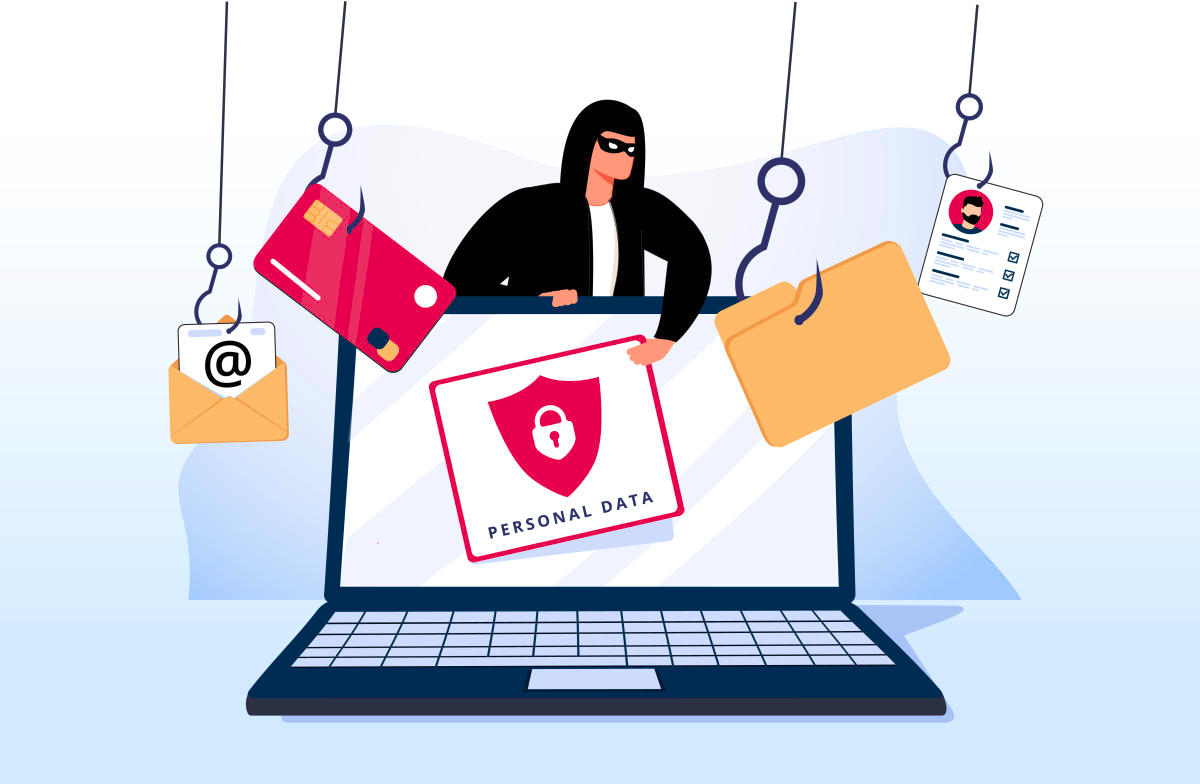
\includegraphics[width=\textwidth]{img/phishing.png}
Phishing, que é um termo como Fishing, pescando em inglês, porém a grafia diferente é utilizada paenas para a ameaça social. Esta é uma das técnicas de ameaça virtual que utiliza Engenharia Social, ou seja, um Hacker atacante se utiliza de uma análise social da vítima para tirar proveito dela e atacá-la. O Phishing traz alguma forma de enganação para a vítima clicar em um link controlado pelo atacante para uma futura ação.

\begin{ficadica}
Esta é uma ameaça de entrada para futuras ações que o atacante utlizará para prejudicar a vítima.
\end{ficadica}

Por se tratar de uma técnica de Engenharia Social e muitas vezes ser passada através de email, a prevenção deste ataque é apenas de cautela. Sempre deve-se ficar atento quando um link para algum acesso delicado é fornecido, algum tipo de banco ou site de comercio online, estes ataques sempre vão se renovando e se sofisticando. A principal chave para não ser enganado é conferir as informações e elementos de mensagem com os meios oficiais de quem envia, ficando atento se a mensagem se mostra ser de fato profissional, muitas vezes as mensagens falsas possuem designs diferentes ou erros de ortografia.

\section{Spoofing}

O Spoofing é uma prática de Fraude, porém no meio digital. Ele pode ser realizado de diversas formas e visa confundir uma vítima passando uma criação de um Hacker atacante como se fosse algo original, podendo ocorrer em sites, aplicativos, emails e mensagens.

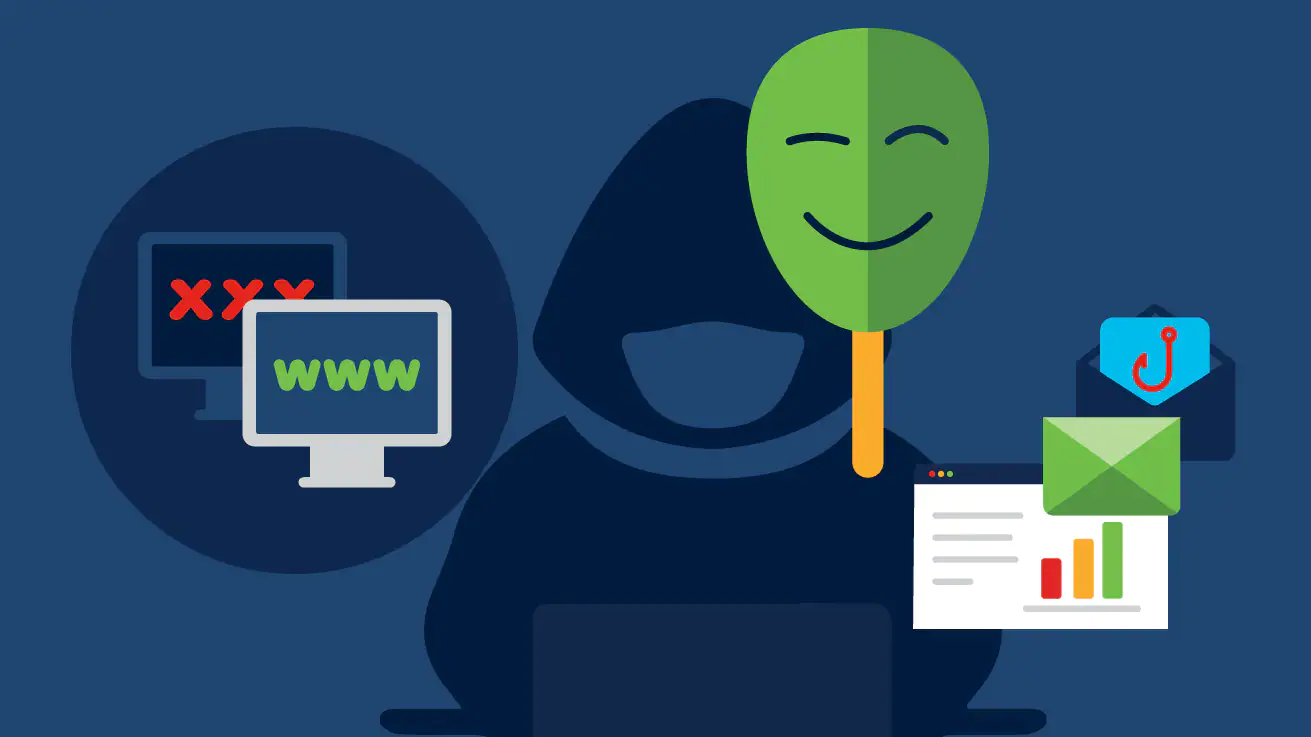
\includegraphics[width=\textwidth]{img/spoofing.png}

Emails de Spoofing são muito comuns e trazem uma aparência próxima à mensagens autênticas. Tais mensagens podem ocultar links de Phishing ou então programas maliciosos como Spywares, vírus, worm, entre outros.

Além dos emails, também há o spoofing em sites. Os Hackers utilizam nomes de sites muito parecidos com os originais porém com conteúdos feitos por eles podendo assim adquirir dados sensíveis como senhas de algum cliente enganado pela ameaça.


\section{Spyware}
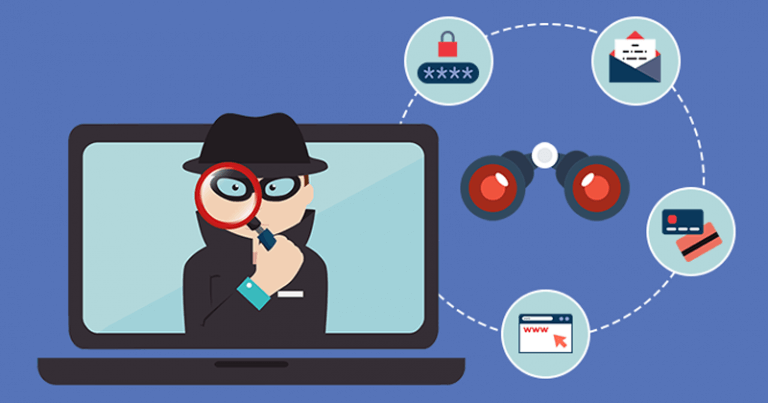
\includegraphics[width=\textwidth]{img/spyware.png}
Spyware, nome que vem de Software Espião, é um tipo de ameaça que registra informações pessoais de algum computador ou celular e passa essas informações para o criador do Spyware. Este registro de informações pode ser realizado de diversas formas, como o keylog que registra apenas os botões acionados pelo usuário, o screenlog que registra tudo o que aparece na tela da vitima da ameaça. A ameaça é perigosa quando o usuário acessa programas ou dados sensíveis, podendo revelar senhas ou dados de acesso restrito para o atacante por meio do programa instalado na máquina.

O Spyware normalmente entra num aparelho a partir de métodos como os explicados acima, phishing ou spoofing podem ser meios para um hacker adicionar um spyware no computador. O primeiro método de proteção é ficar atento a etas ameaças. Porém é sempre importante ter um anti-virus que pode detectar a presença de um destes softwares maliciosos em seu aparelho e retirá-lo.

\begin{atencao}
Uma ferramenta confiável pra descobrir se o site é autêntico é a certificação digital. Este é o cadeado no lado esquerdo do do campo de url, é possível clicar nele e averiguar mais sobre a identidade do site
\end{atencao}

\section{Resumo}
Nesse capítulo estudamos algumas ameaças concretas que podem atacar a segurança da informação pessoal e como nos prevenir delas. Foram elas: Phishing, Spoofing e Spyware.bÉ importante ter esse conhecimento e aplicar suas prevenções sempre no dia a dia.


\chapter{Exercícios}

\subsection*{Exercício 1}

O que é engenharia social e como ela perigosa para a segurança da informação?

\subsection*{Exercício 2}

Quais são as melhores medidas para não ser vítima de ameaças de segurança da informação pessoais?
